\documentclass[twoside,12pt,a4paper,titlepage]{article}

\usepackage{xspace}
\usepackage{siunitx}
\usepackage{booktabs}
\usepackage{rotating}
\usepackage[margin=2.3cm]{geometry}
\usepackage{gensymb}

\newcommand{\org}{SourceBots\xspace}
\newcommand{\staff}{SourceBots staff\xspace}
\newcommand{\gamename}{Tin Can Rally\xspace}
\newcommand{\timeline}{August 2018\xspace}

\title{\gamename}
\author{\org}
\date{\timeline}

\usepackage{helvet}
\renewcommand{\familydefault}{\sfdefault}

\usepackage[pdftex,
            hidelinks]{hyperref}

\begin{document}

\begin{titlepage}
\begin{center}
\includegraphics[width=0.55\textwidth]{./fig-sourcebots.pdf}~\\[1cm]
\textsc{\large SourceBots}~\\[1.8cm]
\includegraphics[width=0.55\textwidth]{./soton_logo.eps}~\\[1cm]
\textsc{\large Electronics and Computer Science}\\[0.2cm]
\textsc{\large Faculty of Engineering and Physical Sciences}\\[0.2cm]
\textsc{\large University of Southampton}\\[1.8cm]
\includegraphics[width=0.55\textwidth]{./smallpeice_logo.jpg}~\\[0.2cm]
\textsc{\large The Smallpeice Trust}\\[1.8cm]
\textsc{\huge \textbf{\gamename{}: Rules}}\\[1cm]
\textsc{\large \timeline}\\[1.2cm]
\textsc{\Large Computing, Electronics, and Robotics}
\end{center}
\end{titlepage}

\section{Game Rules}
\label{sec:rules}

\begin{enumerate}
  \item The game, called \emph{\gamename}, is played in the arena defined in
        Specification~\ref{spec:arena}. The objective is to race around a
        track, picking up cans along the way.
  \item A point is awarded each time a robot crosses a track boundary in a
        clockwise direction. Points are not awarded for re-crossing a track
        boundary which has previously reversed over.
  \item Robots can pick up tin cans which are in the track. Each time a robot
        crosses a track boundary and is awarded a track boundary point, it is
        awarded 1 bonus point for each tin can it is carrying.
  \item At the end of a match, each robot is awarded one additional point for
        each tin can it is carrying.
  \item A robot is deemed to have passed a track boundary when the back of the
        robot passes the line.
  \item Participating teams must present their robots to match officials at
        least one minute before the start of each match.
  \item There will be 2 robots in each match.
  \item \org may have any number of match officials within the arena, including
        during the course of matches.
  \item At the start of each match, robots must be entirely within their
        starting zones.
  \item At the start of each match, teams will be permitted to lean into the
        arena and start their robots.
  \item Each match lasts $180$ seconds.
  \item Teams may be disqualified from one or all matches by match officials,
        for non-compliance with regulations, lateness to the match, or any other
        reason at the discretion of the judge. Teams disqualified before the
        start time of a match will not be permitted to enter a robot.
\end{enumerate}


\clearpage
\section{Regulations}
\label{sec:regs}

\begin{enumerate}
\item The Judge's decision is final.
\item Any assistance from \staff is provided without guarantees.
\item Competitors are expected to behave within the spirit of good
      sporting conduct.
\item All robots must be fully autonomous once started. No remote control
      systems are permitted.
\end{enumerate}

\clearpage
\section{Specifications}
\label{sec:specs}
\newcounter{SpecID}

\subsection{Arena}
\refstepcounter{SpecID}
\label{spec:arena}

\begin{enumerate}
  \item The arena floor is an \SI{9}{m} $\times$ \SI{9}{m} rectangle. The
        tolerance of these two dimensions is $\pm$ \SI{250}{mm}.
  \item The floor of the arena is carpeted.
  \item The layout of the arena is given in Figure~\ref{fig:arena}. This
        figure is to scale.
  \item The outer walls of the arena are at least \SI{600}{mm} high, and the
        interior surface is white plastic-coated hardboard.
  \item The raised area is \SI{2.4}{m} $\times$ \SI{2.4}{m} $\pm$ \SI{100}{mm},
        with a height of \SI{180}{mm} $\pm$ \SI{10}{mm}.
  \item The scoring zones extend a further \SI{2.4}{m} $\times$ \SI{2.4}{m} $\pm$ \SI{100}{mm}
        from the raised area, resulting in a total size of \SI{4.8}{m} $\times$ \SI{4.8}{m} $\pm$ \SI{200}{mm}.
  \item Scoring zones will be bounded by metallic tape around the perimeter
        and internal boundaries. The inside edge of the tape marks the outside
        edge of the scoring zone.
  \item At the cardinal points of the arena are \SI{1.2}{m} $\times$ \SI{1.2}{m} $\pm$ \SI{100}{mm} walls,
        raised at least \SI{180}{mm} $\pm$ \SI{10}{mm}.
  \item Scoring zones for teams will be offset 90\degree{} anti-clockwise, such
        that a team isn't directly in front of their own scoring zone.
  \item Each robot will be assigned a corner at the start of every match to indicate its starting area.
        Corner starting areas are \SI{1000}{mm} $\pm$ \SI{20}{mm} square and will be marked by tape.
\end{enumerate}

\begin{figure}
  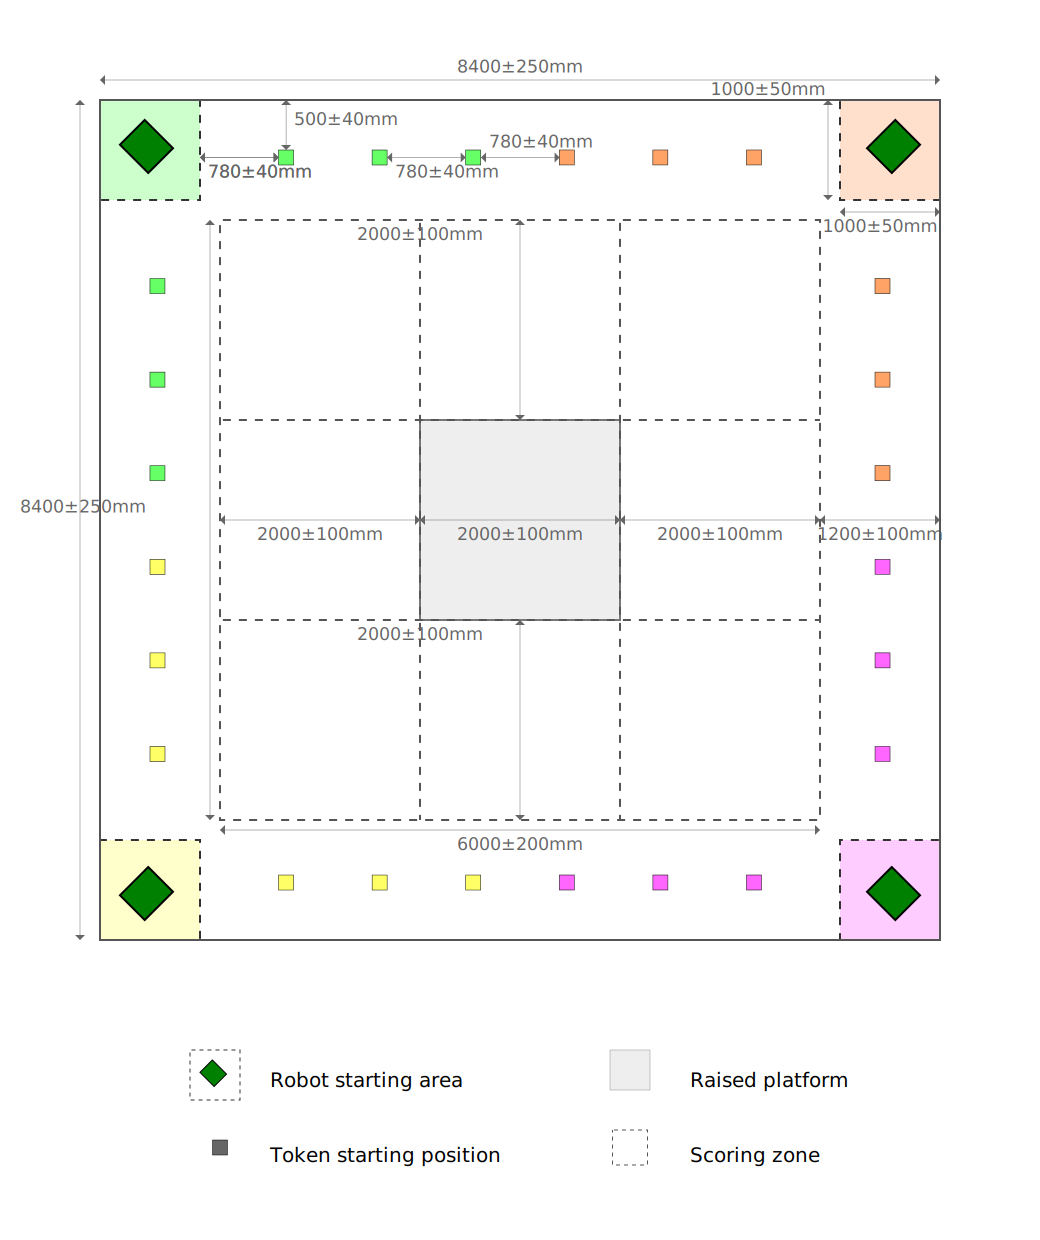
\includegraphics[scale=0.58]{fig-arena.pdf}
  \caption{Layout zones and tokens in the arena.}
  \label{fig:arena}
\end{figure}

\subsection{Tokens}
\refstepcounter{SpecID}
\label{spec:tokens}

\begin{enumerate}
  \item The tokens are cuboids with side length \SI{250}{mm} $\pm$ \SI{10}{mm}.
  \item Each face of each token is bordered by \SI{10}{mm} $\pm$ \SI{2}{mm} of
        copper conductive tape.
  \item There are 20 possible starting positions for tokens in the arena. These
        are arranged as indicated in Figure~\ref{fig:arena}.
  \item At the start of each match each quadrant four of the starting positions
        in each quadrant will be occupied. The position nearest the starting
        area of each quadrant will always be occupied.
  \item While the token starting positions are rotationally symmetrical, the
        pattern of which are occupied in any given match may not be.
\end{enumerate}


\end{document}

